\documentclass [12pt]{article}
\setlength{\parindent}{0em}
\setlength{\parskip}{0.25in}
\usepackage{geometry}
\geometry{verbose,letterpaper,tmargin=0.5in,bmargin=1.0in,lmargin=.70in,rmargin=.70in}
\usepackage{graphicx}
\usepackage{amsmath}
\usepackage{amssymb}
\usepackage{amsthm}
\theoremstyle{definition}
\newtheorem{exmp}{Example}[section]
\usepackage{tikz}
\usetikzlibrary{arrows,decorations.pathmorphing,backgrounds,positioning,fit,petri,calc,matrix}
\usepackage{slashbox}
\usepackage{listings}
\usepackage{ dsfont }
\usepackage{ upgreek }
\usepackage{graphicx}
\graphicspath{ {./images/} }


\newcommand{\ket}[1]{| {#1} \rangle}
\newcommand{\bra}[1]{\langle {#1} |}
\newcommand{\braket}[2]{\langle #1 \ | \ #2 \rangle}
\newcommand{\qp}[2]{\langle #1 \ | \ #2 \ | \ #1 \rangle}
\newcommand{\tensor}[2]{ #1 \otimes  #2 }

\definecolor{dkgreen}{rgb}{0,0.6,0}
\definecolor{gray}{rgb}{0.5,0.5,0.5}
\definecolor{mauve}{rgb}{0.58,0,0.82}

\lstset{frame=tb,
  language=Python,
  aboveskip=3mm,
  belowskip=3mm,
  showstringspaces=false,
  columns=flexible,
  basicstyle={\small\ttfamily},
  numbers=none,
  numberstyle=\tiny\color{gray},
  keywordstyle=\color{blue},
  commentstyle=\color{dkgreen},
  stringstyle=\color{mauve},
  breaklines=true,
  breakatwhitespace=true,
  tabsize=3
}

\DeclareMathOperator{\Cspan}{ \CC-span }

\title{Home Work 9}
\author{Madhu Peduri}
\date{04/12/2021}

\begin{document}
\section*{Homework 9}

{\bf 1.1.} What is the dimension of $dim(\mathds{A} + \mathds{B})$ ?

\phantom{1em} {\bf 1.} We have the following definition 

\phantom{1000em} $\mathds{A}$ and $\mathds{B}$ are subspaces and $\mathds{A} + \mathds{B} = \{ \ket{a} + \ket{b}, \ket{a} \in \mathds{A}, \ket{b} \in \mathds{B}\}$

\phantom{1000em} We know that, the dimension of a vector space is the number of vectors in its basis. \\
\phantom{1000em} Let A and B are the basis for $\mathds{A}$ and $\mathds{B}$\\
\phantom{1000em} We know that basis vectors A and B are orthonormal basis, so they are linearly independent.\\
\phantom{1000em} We know that basis vector formed by $A + B$ span the subspaces $\mathds{A} + \mathds{B}$. 

\phantom{1em} {\bf 2.} From above points we can say, \\
\phantom{1000em} $A + B$ is basis for the vector spaces formed by $\mathds{A} + \mathds{B}$\\
\phantom{1000em} $\Rightarrow dim(\mathds{A} + \mathds{B}) = dim(\mathds{A}) + dim(\mathds{B})$

{\bf 1.2.} Show that $\mathcal{P}(\ket{v}, \mathds{A} + \mathds{B}) = \mathcal{P}(\ket{v}, \mathds{A}) + \mathcal{P}(\ket{v}, \mathds{B})$

\phantom{1em} {\bf 1.} If $\ket{v}$ is the state of the input vector, then quantum probability of finding \\
\phantom{1000em} the system in state x is, $\mathcal{P}(\ket{v}, x) = \braket{v}{x}\braket{x}{v} = \qp{v}{\Uppi_{x}}$, where\\
\phantom{1000em} $\Uppi_{x}$ is the orthogonal projection operator on to the subspace spanned by $\ket{x}$\\
\phantom{1000em} $\Uppi_{x} = \sum_{j}\ket{x_{j}}\bra{x_{j}}$

\phantom{1em} {\bf 2.} By above definition, the quantum probability of finding a system in state $\mathds{A} + \mathds{B}$ is\\
\phantom{1000em} $\mathcal{P}(\ket{v}, \mathds{A} + \mathds{B}) =  \qp{v}{\Uppi_{\mathds{A} + \mathds{B}}}$

\phantom{1em} {\bf 3.} From above two points, we know that $\Uppi_{\mathds{A} + \mathds{B}} = \sum_{j}\ket{e_{j}}\bra{e_{j}}$ where $e_{j} \in A + B$\\
\phantom{1000em} We know that basis $\ket{e_{j}}$ is formed by $\ket{a} + \ket{b}$, where $ \ket{a} \in \mathds{A}, \ket{b} \in \mathds{B}$\\
\phantom{1000em} $\Rightarrow \Uppi_{\mathds{A} + \mathds{B}} = \sum_{j}\ket{e_{j}}\bra{e_{j}} = \sum_{n}\ket{a}\bra{a} + \sum_{m}\ket{b}\bra{b}$\\
\phantom{1000em} $\Rightarrow \Uppi_{\mathds{A} + \mathds{B}} = \Uppi_{\mathds{A}} + \Uppi_{\mathds{B}}$

\phantom{1em} {\bf 4.} By point 3, we can rewrite the definition in point 2 as, \\
\phantom{1000em} $\mathcal{P}(\ket{v}, \mathds{A} + \mathds{B}) =  \qp{v}{\Uppi_{\mathds{A} + \mathds{B}}} = \qp{v}{\Uppi_{\mathds{A}} + \Uppi_{\mathds{B}}}$

\phantom{1em} {\bf 5.} Applying the projection operator $\Uppi$ on a state vector is a linear transformation \\
\phantom{1000em} and as it is a vector space homomorphishm, we can say,

\phantom{1000em} $\qp{v}{\Uppi_{\mathds{A}} + \Uppi_{\mathds{B}}} = \qp{v}{\Uppi_{\mathds{A}}} + \qp{v}{\Uppi_{\mathds{B}}}$

\phantom{1000em} $\Rightarrow \mathcal{P}(\ket{v}, \mathds{A} + \mathds{B}) = \mathcal{P}(\ket{v}, \mathds{A}) + \mathcal{P}(\ket{v}, \mathds{B})$

\newpage

{\bf 1.3.} Show that $\Uppi_{\mathds{A}}\Uppi_{\mathds{B}} = \Uppi_{\mathds{B}}\Uppi_{\mathds{A}}$

\phantom{1em} {\bf 1.} We know that,

\phantom{1000em} $\Uppi_{\mathds{A}} = \sum_{i}\ket{a_{i}}\bra{a_{i}}$\\
\phantom{1000em} $\Uppi_{\mathds{B}} = \sum_{j}\ket{b_{j}}\bra{b_{j}}$\\

\phantom{1em} {\bf 2.} $\Uppi_{\mathds{A}}\Uppi_{\mathds{B}}$ will be of the form,

\phantom{1000em} $(\ket{a_{1}}\bra{a_{1}} + \dotsb + \ket{a_{i}}\bra{a_{i}}).(\ket{b_{1}}\bra{b_{1}} + \dotsb + \ket{b_{j}}\bra{b_{j}})$

\phantom{1000em} $\Rightarrow \sum_{i,j}\ket{a_{i}}\bra{a_{i}}\ket{b_{j}}\bra{b_{j}})$

\phantom{1000em} $\Rightarrow \sum_{i,j}\ket{a_{i}}\braket{a_{i}}{b_{j}}\ket{b_{j}}$

\phantom{1000em} But we know that $\mathds{A}, \mathds{B}$ are orthogonal $\Rightarrow \braket{a_{i}}{b_{j}} = 0$

\phantom{1000em} $\Uppi_{\mathds{A}}\Uppi_{\mathds{B}} = \sum_{i,j}\ket{a_{i}}\braket{a_{i}}{b_{j}}\ket{b_{j}} = 0$

\phantom{1em} {\bf 3.} Similarly, $\Uppi_{\mathds{B}}\Uppi_{\mathds{A}} = \sum_{i,j}\ket{b_{j}}\braket{b_{j}}{a_{i}}\ket{a_{i}} = 0$

\phantom{1em} {\bf 4.} From points 2,3 we can say,

\phantom{1000em} $\Uppi_{\mathds{A}}\Uppi_{\mathds{B}} = \Uppi_{\mathds{B}}\Uppi_{\mathds{A}} = 0$
 
\newpage
 
{\bf 2.1.} Show that $\Uppi_{\mathds{A} \otimes \mathds{B}} = \Uppi_{\mathds{A}} \otimes \Uppi_{\mathds{B}}$\\
\phantom{10em}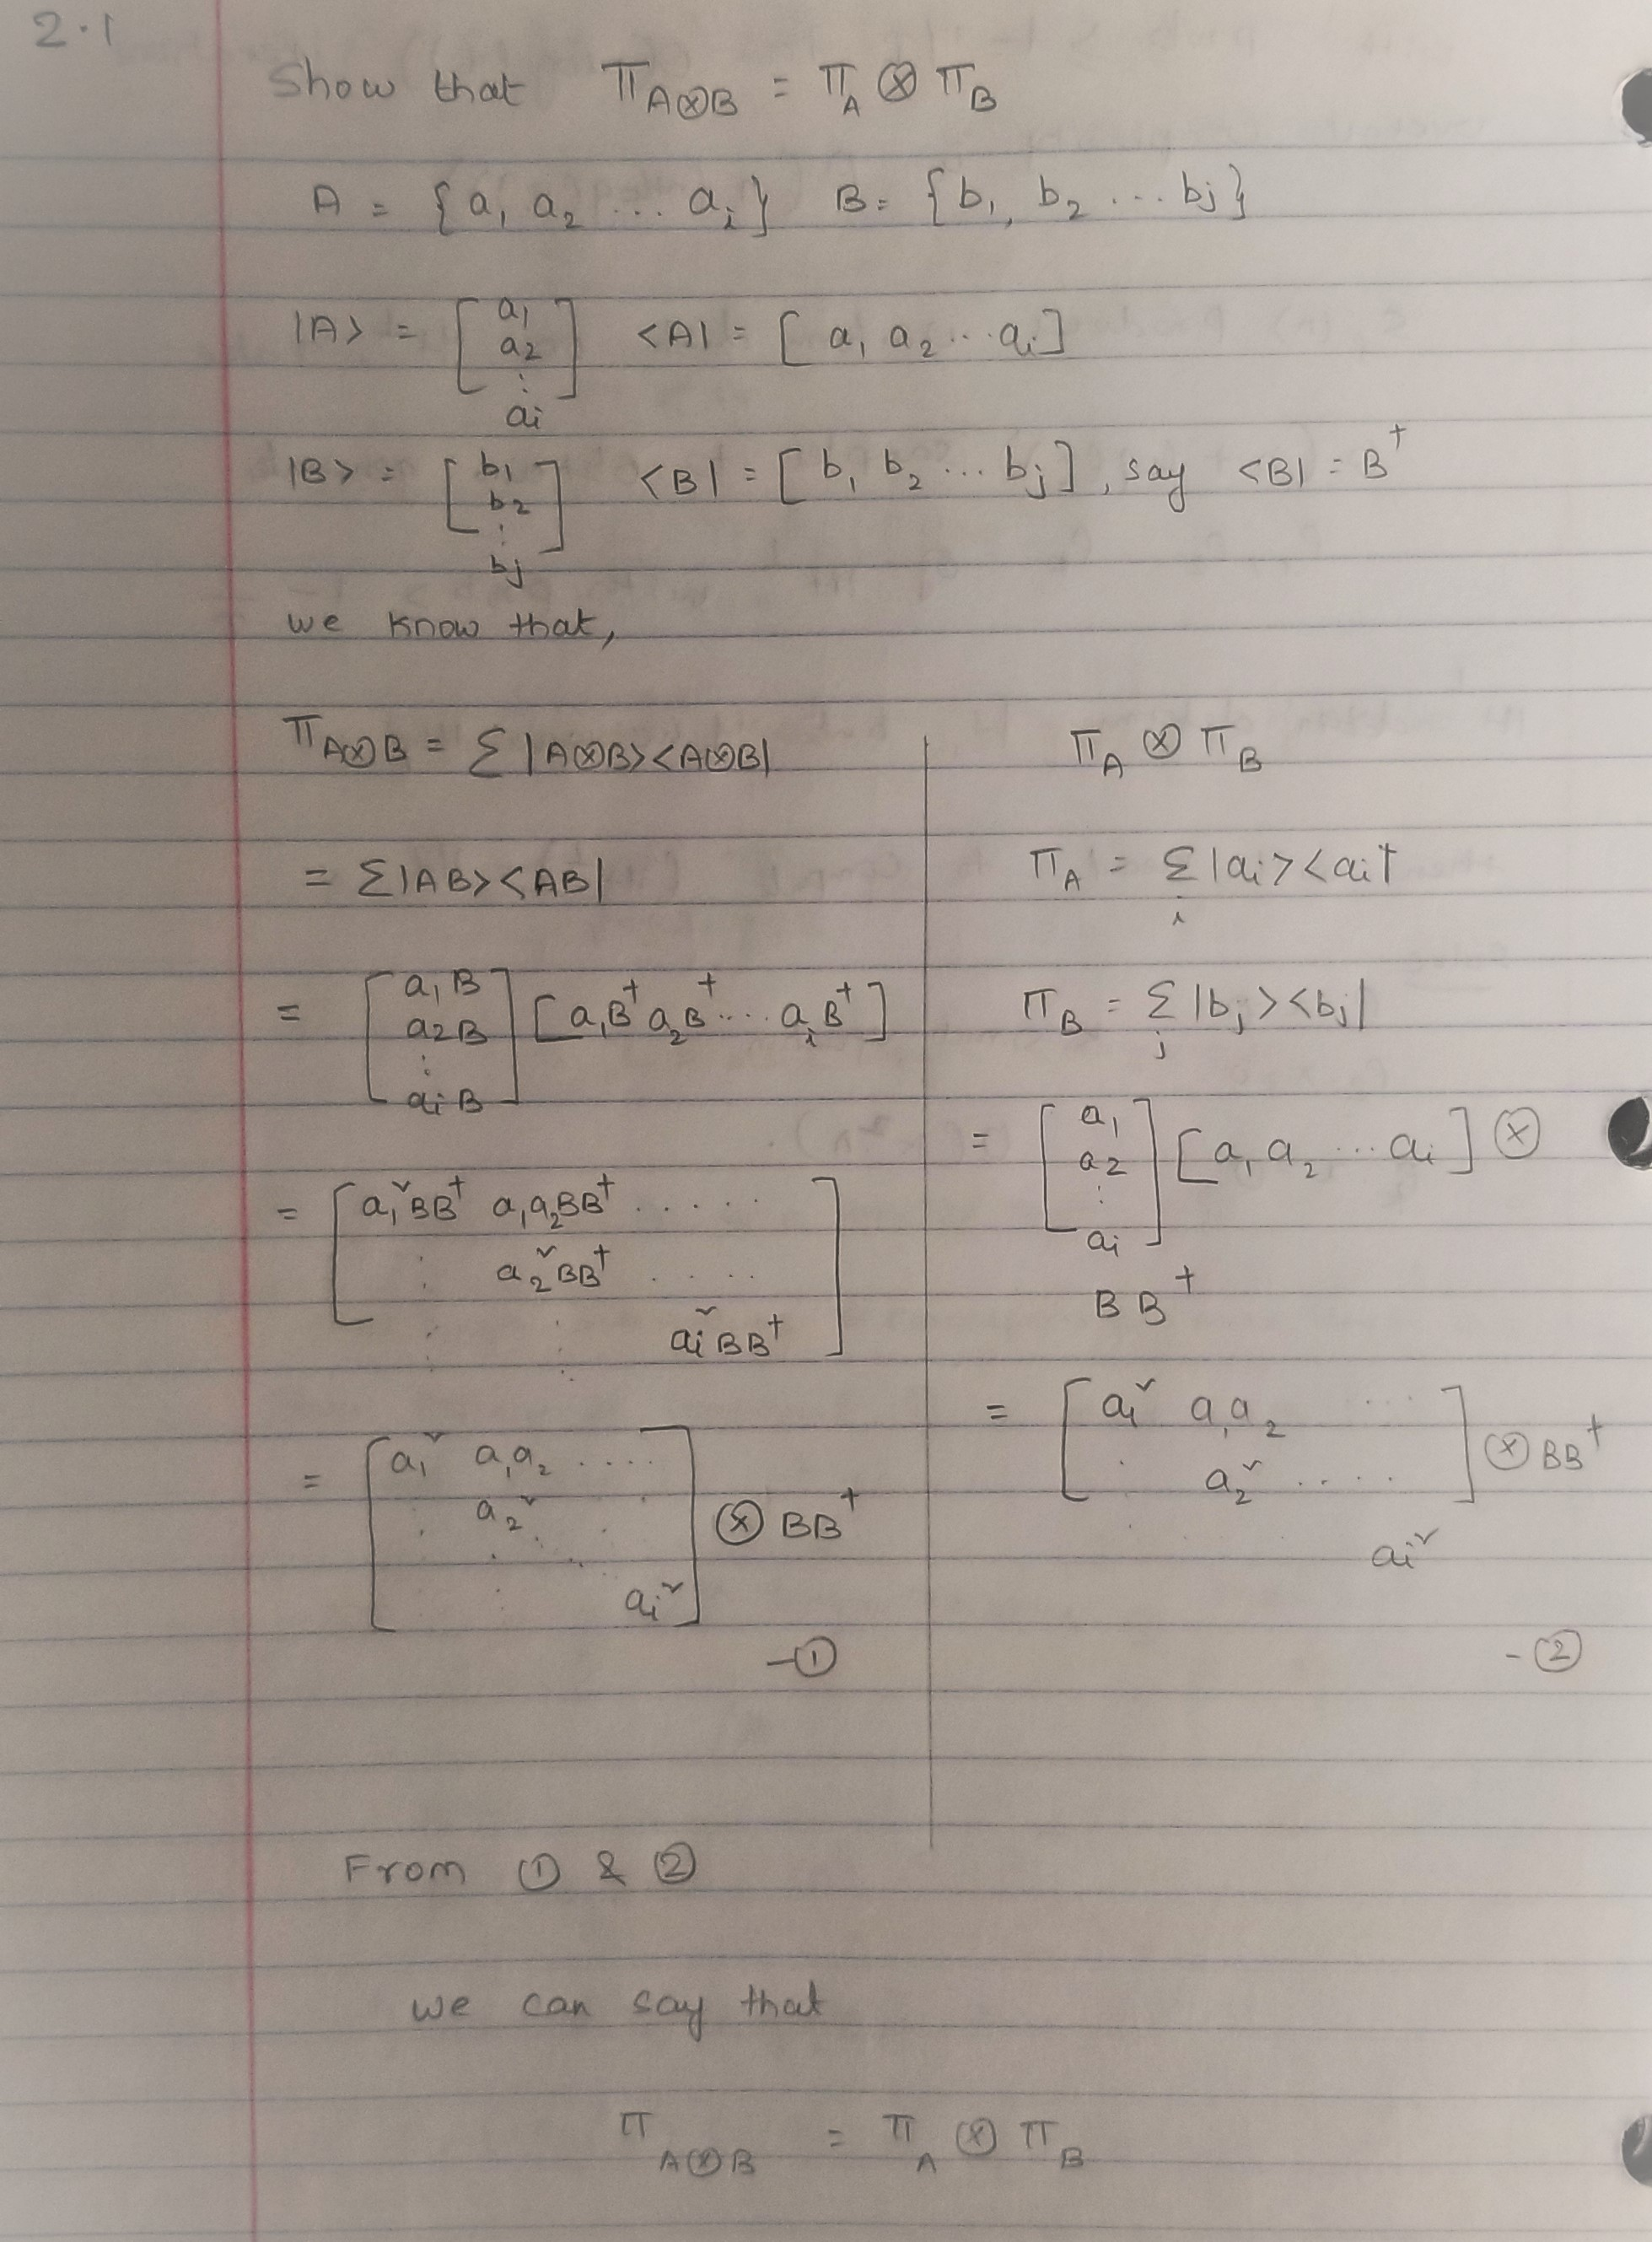
\includegraphics[width=17cm, height=17cm]{I1} 

\newpage

{\bf 2.2.} Show that $\mathcal{P}(\rho \otimes \mathcal{T}, \mathds{A} \otimes \mathds{B}) = \mathcal{P}(\rho, \mathds{A})\mathcal{P}(\mathcal{T}, \mathds{B})$

\phantom{1em} {\bf 1.} Given a quantumn state $\ket{\alpha}$, the density matrix of $\ket{\alpha}$ is its outer product $\ket{\alpha}\bra{\alpha}$

\phantom{1em} {\bf 2.} We know that the probability of observing a state to be in `m', \\
\phantom{1000em} in terms of a density matrix is of the form,

\phantom{1000em} $\mathcal{P}(\ket{\alpha}, m) = \sum_{k}\qp{\alpha_{k}}{\Uppi_{m}}$

\phantom{1000em} $\quad\quad\quad\quad\quad = Tr(\sum_{k}\qp{\alpha_{k}}{\Uppi_{m}})$

\phantom{1000em} $\quad\quad\quad\quad\quad = Tr(\sum_{k}\ket{\alpha_{k}}\bra{\alpha_{k}}\Uppi_{m})$, as Trace is not affected by cyclic permutation.

\phantom{1000em} $\quad\quad\quad\quad\quad = Tr(\rho\Uppi_{m})$, where $\rho$ is the density matrix

\phantom{1em} {\bf 3.} Using above notation, we can say that,

\phantom{1000em} $\mathcal{P}(\rho \otimes \mathcal{T}, \mathds{A} \otimes \mathds{B}) = Tr((\rho \otimes \mathcal{T})\Uppi_{\mathds{A} \otimes \mathds{B}})$

\phantom{1000em} $\quad\quad\quad\quad\quad\quad\quad\quad = Tr((\rho \otimes \mathcal{T})\Uppi_{\mathds{A}} \otimes \Uppi_{\mathds{B}})$, from problem 2.1.

\phantom{1em} {\bf 4.} We know that for a linear transformation, $(p \otimes q)(\ket{r} \otimes \ket{s}) = (p\ket{r})\otimes(r\ket{s})$

\phantom{1em} {\bf 5.} Result from point 3 can be written as,

\phantom{1000em} $\mathcal{P}(\rho \otimes \mathcal{T}, \mathds{A} \otimes \mathds{B}) = Tr(\rho\Uppi_{\mathds{A}} \otimes \mathcal{T}\Uppi_{\mathds{B}})$

\phantom{1000em} $ \quad\quad\quad\quad\quad\quad\quad\quad= Tr(\rho\Uppi_{\mathds{A}})Tr(\mathcal{T}\Uppi_{\mathds{B}})$

\phantom{1000em} $ \quad\quad\quad\quad\quad\quad\quad\quad= \mathcal{P}(\rho, \mathds{A})\mathcal{P}(\mathcal{T}, \mathds{B})$

\end{document}